\chapter{Complexity Theory}

\lecture{12}{2025-12-8}{}

\section{Big-O Notation}

\begin{prev}
    We have dicussed the concept of solvable
    \[
        \text{Decidable} \implies \text{Computationally Solvable}
    \]
\end{prev}

However, not all algorithms are created equal. Some algorithms are more efficient than others. To analyze the efficiency of algorithms, we use \textbf{Big-O Notation}.

\subsection{Analysis of Algorithms}

\begin{itemize}
    \item \textbf{Worst Case}: The maximum number of steps taken by an algorithm for any input of size $n$.
    \item \textbf{Average Case}: The expected number of steps taken by an algorithm for a random input of size $n$.
\end{itemize}

Usually, we focus on the worst-case analysis to ensure that our algorithm performs.

\begin{definition}
    We use a function \[
        f: \mathbb{N} \to \mathbb{R}^+
    \]
    to represent the number of steps.
    \begin{itemize}
        \item $n$: length of input
        \item $f(n)$: number of steps
    \end{itemize}
\end{definition}

Then we give the definition of Big-O notation.

\begin{definition}[Big-O Notation]
    We say \[
        f(n) = O(g(n))
    \]
    if \[
        \exists c > 0, n_0 \in \mathbb{N} \text{ such that } \forall n \geq n_0, f(n) \leq c \cdot g(n)
    \]
\end{definition}

\newpage

Consider the following example.
\begin{eg}
    $f(n) = 6n^3 + 5$
\end{eg}
We have \[
    6n^3 + 5 \leq 7n^3 \text{ for } n \geq 2
\]
That is, we can choose $c = 7$ and $n_0 = 2$. Thus, \[
    f(n) = O(n^3)
\]
Additionally, we can also say $f(n) = O(n^4)$ as \[
    6n^3 + 5 \leq 7n^4 \text{ for } n \geq 2
\]


\begin{eg}
    $f(n) = 3n \log_2 n + 5n \log_2 \log_2 n$
\end{eg}

We can prove that \[
    f(n) = O(n \log n)
\]

\begin{note}
    Note that the base of the logarithm does not matter in Big-O notation since \[
        \log_a n = \frac{\log_b n}{\log_b a} = c \cdot \log_b n = O(\log_b n)
    \]
\end{note}

From \[
    n \leq 2^n, \ \forall n \geq 1
\]
we have \[
    \log_2 n \leq n
\]
From this, we can deduce that \[
    \log_2 \log_2 n \leq \log_2 n
\]
Therefore, \[
    f(n) \leq 3n \log_2 n + 5n \log_2 n = 8n \log_2 n, \ \forall n \geq 1
\]

\begin{lemma}
    \[
        O(n) + O(n^2) = O(n^2)
    \]
\end{lemma}
\vspace{-1em}
\begin{proof}
    Formally, \[
        f(n) = O(n),\ g(n) = O(n^2) \implies f(n) + g(n) = O(n^2)
    \]
    By definition, \[
        \begin{cases}
            \exists c_1, n_1, \ \forall n \geq n_1, f(n) \leq c_1 n \\
            \exists c_2, n_2, \ \forall n \geq n_2, g(n) \leq c_2 n^2
        \end{cases}
    \]
    Then, \[
        f(n) + g(n) \leq c_1 n + c_2 n^2 \leq (c_1 + c_2) n^2, \ \forall n \geq \max(n_1, n_2)
    \]
    Thus, we choose $c = c_1 + c_2$ and $n_0 = \max(n_1, n_2)$
\end{proof}

\newpage

\begin{lemma}[Exponential Function]
    \[
        f(n) = 2^{O(n)}
    \]
    if $\exists\ c, n_0$ such that \[
        f(n) \leq 2^{c \cdot n}, \ \forall n \geq n_0
    \]
\end{lemma}

\begin{lemma}[Constant Function]
    \[
        f(n) = O(1)
    \]
    if $\exists\ c, n_0$ such that \[
        f(n) \leq c \cdot 1, \ \forall n \geq n_0
    \]
    Thus, \[
        f(n) \leq \max\{f(1), \ldots, f(n_0 - 1), c\}, \ \forall n
    \]
    i.e.
    \[
        f(n) \text{ is bounded by a constant for all } n
    \]
\end{lemma}


\subsection{small o Notation}
\begin{definition}[small o Notation]
    We say \[
        f(n) = o(g(n))
    \]
    if \[
        \lim_{n \to \infty} \frac{f(n)}{g(n)} = 0
    \]
\end{definition}

\begin{note}
    Follow the definition of limit, if \[
        \lim_{n \to \infty} f(n) = L
    \]
    then for any $\epsilon > 0$, $\exists \delta$ such that \[
        \forall n > \delta, |f(n) - L| < \epsilon
    \]
    Then, for small o notation, we have \[
        \forall c > 0, \exists n_0 \text{ such that } \forall n \geq n_0,\ \frac{f(n)}{g(n)} \leq(<) c
    \]
\end{note}

\begin{remark}
    $O$ versus $o$:
    \[
        \begin{cases}
            f(n) = O(g(n)) & \text{ if } \exists c > 0, n_0 \text{ such that } \forall n \geq n_0, f(n) \leq c \cdot g(n) \\
            f(n) = o(g(n)) & \text{ if } \forall c > 0, \exists n_0 \text{ such that } \forall n \geq n_0, f(n) < c \cdot g(n)
        \end{cases}
    \]
\end{remark}


\begin{eg}
    Consider \[
        A = \{0^k1^k \mid k \geq 0\}
    \]
    What is the $\#$ steps taken by a one-tape Turing machine to process a string?
\end{eg}

We can separate the process into these steps:

\begin{enumerate}[label=$\arabic*^\circ$]
    \item We have to check if input is \[
        0\ldots0 1\ldots1
    \]
    which takes $O(n)$ steps.
    \item Then, move back, which takes $O(n)$ steps.
    \item Next, we cross off one $0$ and one $1$, which takes $O(n)$ steps.
    \item We repeat steps 2 and 3 until all $0$s and $1$s are crossed off, which has $n/2$ iterations.
\end{enumerate}
Thus, the total number of steps is \[
    O(n) + \frac{n}{2} \cdot O(n) + O(n) = O(n^2)
\]

\begin{definition}[Time Complexity Class]
    \[
        \text{TIME}(t(n)) \equiv \{L \mid \text{a language decided by an } O(t(n)) \text{ TM}\}
    \]
\end{definition}

Now we have \[
    A = \{0^k1^k \mid k \geq 0\} \in \text{TIME}(n^2)
\]
But we can do better: 
We first cross off every other $0$ and then cross off every other $1$. This way, we can do \begin{align*}
    &\underline{0}0\underline{0}0\underline{0}\underline{1}1\underline{1}1\underline{1} \\
    &\underline{0}0
\underline{1}1 \\
    &\underline{0}\underline{1} \\
    &\epsilon
\end{align*}
The key is the length of the string left must be always even.

\begin{algorithm}
\caption{Decide Language $A = \{0^k 1^k \mid k \geq 0 \}$}
\SetKwInput{Input}{Input}
\SetKwInput{Output}{Output}

\Input{String $w$}
\Output{Accept or Reject}
\If{format is not $0^* 1^*$}{
    \Return Reject\;
}
\While{tape contains any 0s or 1s}{
    Scan tape to count total number of active 0s and 1s\;
    \If{total count is Odd}{
        \Return Reject\;
    }   
    \For{each type $x \in \{0, 1\}$}{
        Keep the 1st $x$, cross off the 2nd $x$, keep the 3rd $x$...
    }
}
\Return Accept\;
\end{algorithm}

The whole process takes \[
    1 + \log_2 n
\]
iterations, and each iteration takes $O(n)$ steps. Thus, the total number of steps is \[
    O(n \log n)
\]
Thus, we have \[
    A \in \text{TIME}(n \log n)
\]
We can't do any better than this since

\begin{theorem}
    Any language decided in $o(n \log n)$ time by a one-tape Turing machine is regular.
\end{theorem}

But we know that $A$ is not regular.

\begin{remark}
    If we want to use the method of copying, the problem is that  the copy operation is expensive. It takes $O(n^2)$ times to copy $n$ symbols.
\end{remark}

We can also do an $O(n)$ algorithm using a two-tape Turing machine.
\begin{enumerate}[label=$\arabic*^\circ$]
    \item Check if input is \[
        0\ldots0 1\ldots1
    \] which takes $O(n)$ steps.
    \item Copy all $0$s to the 2nd tape, which takes $O(n)$ steps.
    \item Sequentially match each $1$ on the 1st tape with a $0$ on the 2nd tape, which takes $O(n)$ steps. (if no $0$ left, reject)
    \item If all $1$s are matched, accept; else, reject.
\end{enumerate}

The total number of steps is \[
    O(n) + O(n) + O(n) = O(n)
\]
But this requires a two-tape Turing machine.

\section{Time Complexity}

\begin{prev}
    In Ch.3 we have dicussed the concept of various Turing machines, which are all equivalent in Computability Theory.
\end{prev}

However, in Complexity Theory, different Turing machines may have different time complexities for the same language.

\subsection{Multi-tape TM and Time Complexity}

\begin{theorem}
    Let $t(n) \geq n$. For a $t(n)$ time multi-tape Turing machine, there exists an equivalent $O(t(n)^2)$ time single-tape Turing machine.
\end{theorem}
\vspace{-1em}
\begin{proof}
    Recall the simulation of multi-tape TM by single-tape TM. 
    \begin{figure}[H]
        \centering
        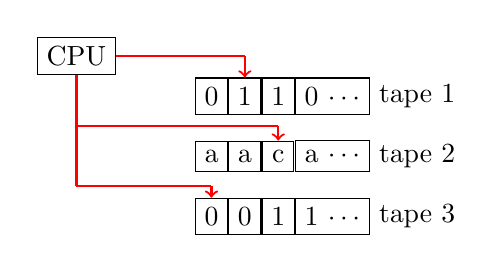
\begin{tikzpicture}[ampersand replacement=\&]
        \matrix 
        {
        \node[draw](0) {CPU}; \& [1cm]  \& \node(1){} ; \&\&\& \\
        \& \node[draw]{0}; \& \node[draw](a){1}; \& \node[draw]{1}; \& \node[draw]{0 $\cdots$};  \& \node{tape 1};\\
        \node(2){} ; \&  \&  \& \node(21){} ; \&\& \\  
        \& \node[draw]{a}; \& \node[draw]{a}; \& \node[draw](b){c}; \& \node[draw]{a $\cdots$}; \&  \node{tape 2}; \\
        \node(3){} ; \& \node(31){} ; \&  \&  \&\& \\
        \& \node[draw](c){0}; \& \node[draw]{0}; \& \node[draw]{1}; \& \node[draw]{1 $\cdots$}; \&  \node{tape 3}; \\
        };

        \draw [-,red,thick] (0) -- (1.center) ;
        \draw [->,red,thick] (1.center) -- (a) ;
        \draw [-,red,thick] (0) -- (2.center) ;
        \draw [-,red,thick] (2.center) -- (21.center) ;
        \draw [->,red,thick] (21.center) -- (b) ;
        \draw [-,red,thick] (0) -- (3.center) ;
        \draw [-,red,thick] (3.center) -- (31.center) ;
        \draw [->,red,thick] (31.center) -- (c) ;
        \end{tikzpicture}
        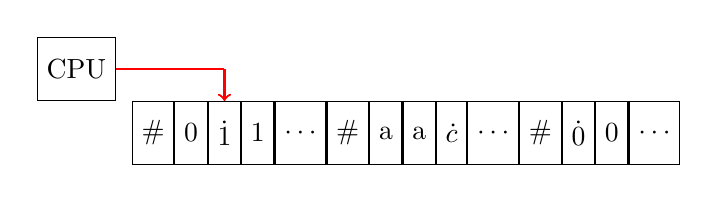
\begin{tikzpicture}[ampersand replacement=\&]
        \matrix[nodes={minimum height=8mm}] 
        {
        \node[draw](0) {CPU}; \& [0.2cm] \& \& \node(1){} ; \& \&\&\& \&\&\& \&\&\& \\
        \& \node[draw]{\#};  \& \node[draw]{0}; \& \node[draw](a){$\dot{1}$}; \& \node[draw]{1}; \& \node[draw]{$\cdots$};
        \& \node[draw]{\#};  \& \node[draw]{a}; \& \node[draw]{a}; \& \node[draw]{$\dot{\text{c}}$}; \& \node[draw]{$\cdots$}; 
        \& \node[draw]{\#};  \& \node[draw](c){$\dot{0}$}; \& \node[draw]{0}; \& \node[draw]{$\cdots$}; \\
        };

        \draw [-,red,thick] (0) -- (1.center) ;
        \draw [->,red,thick] (1.center) -- (a) ;
        \end{tikzpicture}
        \caption{Simulation of Multi-tape TM by Single-tape TM}
    \end{figure}
    To simulate each step of multi-tape TM, we scan to know where heads point to and do the update. However, we have to right shift the tape. Si we need to know the tape length which is \[
        k \times O(t(n)) = O(t(n)) \quad \text{for constant } k
    \]
    A $t(n)$ multi-tape TM generates at most $O(t(n))$ contens in $O(t(n))$ time. Thus, the cost of simulating each step of multi-tape TM is $O(t(n))$. Therefore, the total time is \[
        O(t(n)) \times O(t(n)) = O(t(n)^2)
    \]
\end{proof}

\begin{definition}
    NTM Time Complexity $t(n)$ is the maximum \# steps the machine uses for any path from root to leaf in the computation tree for any input of size $n$.
\end{definition}

\begin{theorem}
    Let $t(n) \geq n$. For a $t(n)$ single-tape NTM, there exists an equivalent $2^{O(t(n))}$ time single-tape TM. 
\end{theorem}
\vspace{-1em}
\begin{proof}
    Assume $b$ is the maximal number of branches at each node. Recall the way to simulate NTM by multi-tape TM.
    \begin{figure}[H]
        \centering
        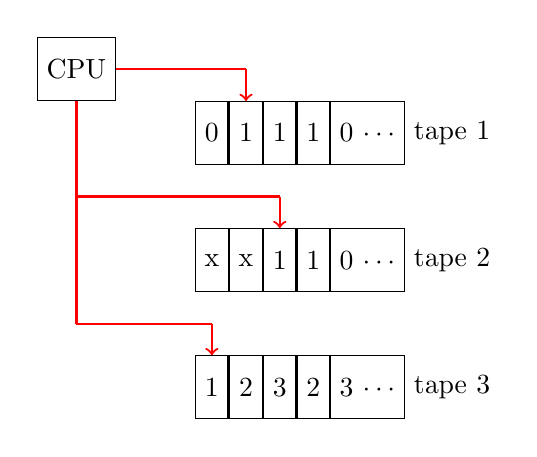
\begin{tikzpicture}[ampersand replacement=\&]
            \matrix[nodes={minimum height=8mm}]     
            {
            \node[draw](0) {CPU}; \& [1cm]  \& \node(1){} ; \&\&\& \& \\
            \& \node[draw]{0}; \& \node[draw](a){1}; \& \node[draw]{1}; \& \node[draw]{1};  \& \node[draw]{0 $\cdots$};  \& \node{tape 1};\\
            \node(2){} ; \&  \&  \& \node(21){} ; \&\& \&\\  
            \& \node[draw]{x}; \& \node[draw]{x}; \& \node[draw](b){1}; \& \node[draw]{1}; \& \node[draw]{0 $\cdots$}; \& \node{tape 2};  \\
            \node(3){} ; \& \node(31){} ; \&  \&\& \& \&\\
            \& \node[draw](c){1}; \& \node[draw]{2}; \& \node[draw]{3}; \& \node[draw]{2}; \& \node[draw]{3 $\cdots$}; \&  \node{tape 3}; \\
            };

            \draw [-,red,thick] (0) -- (1.center) ;
            \draw [->,red,thick] (1.center) -- (a) ;
            \draw [-,red,thick] (0) -- (2.center) ;
            \draw [-,red,thick] (2.center) -- (21.center) ;
            \draw [->,red,thick] (21.center) -- (b) ;
            \draw [-,red,thick] (0) -- (3.center) ;
            \draw [-,red,thick] (3.center) -- (31.center) ;
            \draw [->,red,thick] (31.center) -- (c) ;
        \end{tikzpicture}
        \caption{Simulation of NTM by Multi-tape TM}
    \end{figure}
    We use BFS to do the simulation in the computation tree. The total nodes in the computation tree, which can be found in the tape 3 (record the path from root to node) is \[
        1 +  b + b^2 + \cdots + b^{t(n)} = \sum_{i=0}^{t(n)} b^i = O(b^{t(n)})
    \]
    Cost of running from root to one node in tape 2 is $O(t(n))$, and the cost of updating tape 3 is also $O(t(n))$. Thus, the total cost of simulating each node is \[
        \# \text{ nodes} \times \text{ cost per node } = O(b^{t(n)}) \times O(t(n)) = 2^{O(t(n))}
    \]
    \begin{note}
        that \[
            b^{t(n)} \times t(n) = 2^{\log_2 (b^{t(n)}t(n))} = 2^{t(n) \log_2 b + \log_2 t(n)} = 2^{O(t(n))}
        \]
    \end{note}
    This is by the three-tape TM simulating the NTM. By the previous theorem, we can simulate the three-tape TM by a single-tape TM in \[
        (2^{O(t(n))})^2 = 2^{O(t(n))}
    \]
\end{proof}

\newpage

\section{Languages in P}

\begin{definition}[Class P]
    \[
        \text{P} \equiv \bigcup_{k} \text{TIME}(n^k)
    \]
    i.e. the class of languages decidable by a polynomial-time deterministic Turing machine.
\end{definition}

\begin{note}
    $P$ class is roughly the class of solvable problems in computer.
\end{note}

\subsection{PATH Problem}

\begin{eg}
    \[
        \text{PATH} = \{\langle G, s, t \rangle \mid G \text{ is a directed graph s.t. } \exists \text{ path from } s \text{ to } t \}
    \]
\end{eg}

We can prove that \[
    \text{PATH} \in \text{P}
\]

\begin{intuition}
    Let's start with a brute force way
    \begin{enumerate}[label=$\arabic*^\circ$]
        \item $m: |V(G)|$
        \item $|\text{path}| \leq m$ (since no loop)
        \item $\#$paths $\leq m^m$
        \item sequentially check if on has $s$ to $t$ 
    \end{enumerate}
    Total time: \[
        O(m^m \cdot m) = O(m^{m+1})
    \]
    which is exponential time.
\end{intuition}

For an input $\langle G, s, t \rangle$, we can use the following algorithm including $V(G), E(G)$
\begin{enumerate}[label=$\arabic*^\circ$]
    \item Mark $s$
    \item Repeat until no new node is marked:
    \begin{itemize}
        \item For each edge $(u, v) \in E(G)$, if $u$ is marked, mark $v$
    \end{itemize}
    \item If $t$ is marked, accept; else, reject.
\end{enumerate}

$\#$ steps in the main loop is at most $|V|$ (if no newly marked node, we stop). at each iteration, we have to scan $|E| \leq |V|^2$. The cost to mark node is polynomial. Thus, the total time is \[
    O(|V|) \times O(|E|) = O(|V|^3)
\]
Therefore, \[
    \text{PATH} \in \text{P}
\]

\subsection{Relatively Prime Problem}

\begin{definition}[Relatively Prime]
    Let $x, y \in \mathbb{Z}$. We say $x$ and $y$ are \textbf{relatively prime} if their greatest common divisor (gcd) is 1, i.e., \[
        \gcd(x, y) = 1
    \]
\end{definition}

\begin{eg}
    \[
        \text{RELPRIME} = \{\langle x, y \rangle \mid x, y \in \mathbb{N} \text{ are relatively prime} \}
    \]
\end{eg}

From the definition, we have to find a way to compute $\gcd(x, y)$ efficiently. We can use the Euclidean Algorithm.

\begin{algorithm}
\caption{Euclidean Algorithm}
\SetKwInOut{Input}{Input}
\SetKwInOut{Output}{Output}

\Input{$\langle x, y \rangle$}
\Output{Greatest Common Divisor of x and y}

\While{$y \neq 0$}{
    $x \leftarrow x \bmod y$\;
    exchange $x$ and $y$\;
}

\Return{$x$}\;
\end{algorithm}

\begin{note}
    If $x < y$, then in the first iteration, we have \[
        x \leftarrow x \bmod y = x
    \]
    and then exchange $x$ and $y$. Thus, after the first iteration, we have $x \geq y$.
\end{note}

At each iteration, $x$ or $y$ is reduced by at least half.
\begin{itemize}
    \item If $x > y$ \[
        x \bmod y \leq \frac{x}{2}
    \]
    \begin{itemize}
        \item If $x < 2y$, then \[
            x \bmod y = x - y < x - \frac{x}{2} = \frac{x}{2}
        \]
        \item If $x \geq 2y$, then \[
            x \bmod y \leq y \leq \frac{x}{2}
        \]
    \end{itemize}
\end{itemize}

Therefore, \[
    \text{\# iterations} \leq 2 \max(\log_2 x, \log_2 y) = O(n)
\]
where $n$ is the length of the input ($x, y$ are stored as bit string), $\log_2 x + \log_2 y = O(n)$.

In each iteration, $x \bmod y$ is polynomial time computable. Exhanging $x$ and $y$ is also polynomial time. Thus, the total time is \[
    O(n) \times \text{poly}(n) = \text{poly}(n)
\]

\begin{theorem}
    \[
        \text{Context Free Language} \subseteq \text{P}
    \]
\end{theorem}
\vspace{-1em}
\begin{proof}
    Recall the CYK algorithm for CFLs in CNF. For an input string of length $n$, the total time is \[
        O(n^3)
    \]
\end{proof}

\newpage

\section{Languages in NP}

\subsection{Hamiltonian Path Problem}

For some problems, it is difficult to find an algorithm in P. Consider the following example.

\begin{definition}[Hamiltonian Path]
    A \textbf{Hamiltonian Path} in a directed graph is a path that visits all vertex exactly once.
\end{definition}

\begin{figure}[H]
    \centering
    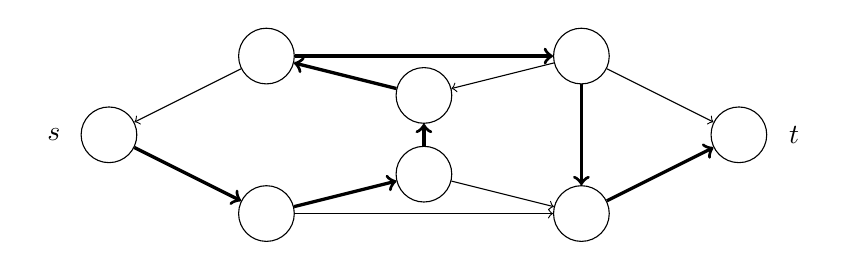
\begin{tikzpicture}[inner sep=2.5mm]      
    \path ( 0,1) node (0) [shape=circle,draw] {}
    (2,2) node (1) [shape=circle,draw] {}
    (2,0) node (2) [shape=circle,draw] {}
    (4,1.5) node (3) [shape=circle,draw] {}
    (4,0.5) node (4) [shape=circle,draw] {}
    (6,2) node (5) [shape=circle,draw] {}
    (6,0) node (6) [shape=circle,draw] {}
    (8,1) node (7) [shape=circle,draw] {};
    \path ( -0.7,1) node {$s$};
    \path ( 8.7,1) node {$t$};
    \draw [->] (1) -- (0);
    \draw [->] (5) -- (3);
    \draw [->] (5) -- (7);
    \draw [->] (2) -- (6);
    \draw [->] (4) -- (6);
    \draw [->, very thick] (4) -- (3);
    \draw [->, very thick] (0) -- (2);
    \draw [->, very thick] (3) -- (1);
    \draw [->, very thick] (1) -- (5);
    \draw [->, very thick] (5) -- (6);
    \draw [->, very thick] (2) -- (4);
    \draw [->, very thick] (6) -- (7);
    \end{tikzpicture}
    \caption{Hamiltonian Path Example}
\end{figure}

\begin{eg}
    \[
        \text{HAMPATH} = \{\langle G, s, t \rangle \mid G: \text{a directed graph with a Hamiltonian path from } s \text{ to } t \}
    \]
\end{eg}

A brute-force way: checking all possible paths, but the number is exponential. So we can do a \textbf{polynomial-time verification} instead.\[
    \text{for a path, in P time} \implies \text{a Hamiltonian path or not}
\]

\subsection{Compositeness Problem}

\begin{definition}[Compositeness]
    We say $x \in \mathbb{N}$ is \textbf{composite} if $\exists\ p, q \in \mathbb{N}$ such that \[
        x = p \cdot q, \quad 1 < p, q < x
    \]
\end{definition}

Given $x$, it is difficult to find such $p, q$ efficiently. However, if we are given $p, q$, we can verify it in polynomial time by multiplication. \\

However, there are still some problems that are difficult to verify in polynomial time, such as the \textbf{Graph Isomorphism Problem}, or the complement of Hamiltonian path problem \[
    \overline{\text{HAMPATH}} = \{\langle G, s, t \rangle \mid G: \text{a directed graph without a Hamiltonian path from } s \text{ to } t \}
\]
Verification is difficult since we have to check all possible paths.

\subsection{Verifier}

\begin{definition}[Verifier]
    An algorithm $V$ is called a \textbf{verifier} for a language $L$ if \[
        L = \{ w \mid \exists c \text{ (certificate) such that } V \text{ accepts } \langle w, c \rangle \}
    \]
\end{definition}

\begin{eg}
    Compositeness problem: $V$ accepts \[
        \langle w, c \rangle = \langle x, p \rangle, \text{ where } p \text{ is a factor of } x
    \]
\end{eg}

\begin{eg}
    HAMPATH problem: $V$ accepts \[
        \langle w, c \rangle = \langle \langle G, s, t \rangle, \text{ path from } s \text{ to } t \rangle
    \]
\end{eg}

$c$ is called a \textbf{certificate} or \textbf{witness} that helps to verify $w \in L$.

\begin{definition}[Polynomial-time Verifier]
    A verifier $V$ is called a \textbf{polynomial-time verifier} if $V$ runs in polynomial time with respect to $|w|$.
\end{definition}

\begin{remark}
    Note that the running time of $V$ is with respect to $|w|$, not $|c|$. For a polynomial-time verifier, we have \[
        |c| \in \text{poly}(|w|)
    \]
    otherwise, $V$ reading $c$ alone would take super-polynomial time.
\end{remark}

\subsection{Class NP}

\begin{definition}[Class NP]
    \[
        \text{NP} \equiv \{ L \mid L \text{ has a polynomial-time verifier} \}
    \]
\end{definition}

Another equivalent definition of NP is as follows.

\begin{definition}[NTIME class]
    \[
        \text{NTIME}(t(n)) = \{ L \mid L \text{ is decidable by a } O(t(n)) \text{ nondeterministic TM}\}
    \]
\end{definition}

\begin{theorem}
    \[
        \text{NP} = \bigcup_{k} \text{NTIME}(n^k)
    \]
\end{theorem}

\vspace{1em}

For the NTM for language $\text{HAMPATH}$, we do 
\begin{enumerate}[label=$\arabic*^\circ$]
    \item Nondeterministically get a path from $s$ to $t$ in the list $p_1\cdots p_m$
    \item For each list:
    \begin{itemize}
        \item Check for repetitions.
        \item Check if each edge $(p_i, p_{i+1})$ exists in $G$.
        \item Check if $s = p_1$ and $t = p_m$
    \end{itemize}
\end{enumerate}

Cost on each list is polynomial. The repetitions cost $O(m^2)$, checking edges cost $O(m^2)$, checking $s$ and $t$ cost $O(m)$. Thus, the total time is \[
    O(m^2) + O(m^2) + O(m) = O(m^2)
\]
Therefore, \[
    \text{HAMPATH} \in \text{NTIME}(n^2) \implies \text{HAMPATH} \in \text{NP}
\]

\newpage

\subsection{NP $\equiv$ Polynomial-time NTM}


\begin{theorem}
    \[
        \bigcup_{k} \text{NTIME}(n^k) = \{L \mid L \text{ decide by a polynomial-time NTM} \}
    \]
\end{theorem}
\vspace{-1em}
\begin{proof}
    We start from the definition:
    \begin{idea}
        We consider both directions.
        \begin{itemize}
            \item[``$\implies$''] NTM by guessing certificate.
            \item[``$\impliedby$''] using NTM’s accepting branch as certificate.
        \end{itemize}
    \end{idea}
    
    \begin{itemize}
        \item[``$\implies$''] Recall the definition of NP. \[
            L = \{ w \mid \exists c \text{ (certificate) such that } V \text{ accepts } \langle w, c \rangle \}
        \]
        We have \[
            |c| \in \text{poly}(|w|) \implies |c| \leq |w|^k
        \]
        because to handle $\langle w, c \rangle$ in $|w|^k$, $|c|$ should be bounded by polynomial of $|w|$. \\
    
        Then we use NTM to 
        \begin{enumerate}[label=$\arabic*^\circ$]
            \item Nondeterministically guess $c$ with length $\leq |w|^k$.
            \item Simulate $V$ on input $\langle w, c \rangle$.
        \end{enumerate}
        That is, we run all $c$ in parallel and each is polynomial time. We have that for any $w \in L$, the NTM accepts in polynomial time. Thus, \[
            L \in \text{NTIME}(n^k)
        \]
        \item[``$\impliedby$''] Assume \[
            L \in \text{NTIME}(n^k)
        \]
        i.e. $w$ is accepted by a polynomial NTM. We let $c$ be any accepting branch where each branch is polynomial time. Then we run the verifier $V$ that handles $\langle w, c \rangle$ in polynomial time. Thus, \[
            L \text{ has a polynomial-time verifier}
        \]
    \end{itemize}
    Proof complete.
\end{proof}

\subsection{SUBSET-SUM Problem}

\begin{eg}
    \[
        \text{SUBSET-SUM} = \left\{ \langle S, t \rangle \;\middle|\; \exists\ S' \subseteq S \text{ such that } \sum_{x \in S'} x = t \right\}
    \]
\end{eg}

Note that we allow repetition of elements in $S$. We will prove that \[
    \text{SUBSET-SUM} \in \text{NP}
\]
Consider any input $\langle \langle S, t \rangle, c \rangle$. We 
\begin{enumerate}[label=$\arabic*^\circ$]
    \item Check if $\sum c_i = t$
    \item Check if $c_i \in S$
    \item If both hold, accept; else, reject.
\end{enumerate} 

The cost of summation is $O(|S|)$, and checking $c_i \in S$ also takes $O(|S|)$. Thus, the total time is \[
    O(|S|) + O(|S|) = O(|S|)
\]
Therefore, \[
    \text{SUBSET-SUM} \in \text{NP}
\]

\subsection{P versus NP and NP-completeness}

Roughly \begin{itemize}
    \item $\text{P}$: problems that can be \textbf{solved} in polynomial time.
    \item $\text{NP}$: problems that can be \textbf{verified} in polynomial time.
\end{itemize}

The greatest open question in computer science is whether \[
    \text{P} = \text{NP}\ ?
\]

It has shown that \[
    \text{P} \subseteq \text{NP}
\]. However, it is not known whether \[
    \text{P} = \text{NP} \text{ or } \text{P} \neq \text{NP}
\]
For certain problems in NP, if we can find a polynomial time algorithm to solve one of them, \[
    \text{P} = \text{NP}
\]
These problems are called \textbf{NP-complete} problems. We will discuss NP-completeness in the next lecture.